% !TEX TS-program = xelatex
% !TEX encoding = UTF-8
%
%
\documentclass[a4paper,12pt]{article}
\usepackage{ctex}
\usepackage{geometry,anysize,changepage,calc,hyperref,cite,fancyhdr,setspace}
\usepackage{amsmath,amssymb,amsthm,listings,xcolor}
\usepackage{graphicx,wrapfig,multirow,diagbox,caption, subcaption,verbatim}
\usepackage{caption,algorithm,algpseudocode}
\usepackage{url,natbib}
\usepackage{wrapfig}
\bibliographystyle{abbrvnat}
\setcitestyle{open={(},authoryear,close={)}}
\renewcommand{\algorithmicrequire}{\textbf{输入}}
\renewcommand{\algorithmicensure}{\textbf{输出}}
\floatname{algorithm}{子程序}
\listfiles
%initialset.tex
%
\hypersetup{bookmarksopen=true,colorlinks=true,linkcolor=red,anchorcolor=blue,citecolor=green,linktocpage=true}
\captionsetup{font=footnotesize}
\captionsetup[sub]{font+=footnotesize}
\linespread{1.5}
\marginsize{2.13cm}{2.14cm}{2.4cm}{2.4cm}
\pagestyle{fancy}
\lstset{xleftmargin=1.5em,xrightmargin=1.5em,frame=lines}%,numbers=left,numberstyle=\tiny}
\chead{}\rhead{\thepage}\lhead{\leftmark}\cfoot{}\rfoot{}\lfoot{}

\newcommand{\vp}{\varphi}
\newcommand{\al}{\alpha}
\newcommand{\be}{\beta}
\newcommand{\ti}{\tilde}
\newcommand{\ve}{\varepsilon}
\newcommand{\de}{\delta}
\newcommand{\na}{\nabla}
\newcommand{\pd}{\partial}
\newcommand{\ud}{\mathrm{d}}
\newcommand{\mr}{\mathrm{R}}
\newcommand{\ms}{\mathbb{S}}
\newcommand{\mz}{\mathbb{Z}}
\newcommand{\mn}{\mathbb{N}}
\newcommand{\mc}{\mathbb{C}}
\newcommand{\one}{\textbf{1}}
\newcommand{\prox}{\textbf{prox}}
\DeclareMathOperator*{\argmax}{argmax}
\DeclareMathOperator*{\argmin}{argmin}
%\DeclareMathOperator*{\logg}{log}
%\DeclareMathOperator*{\det}{det}
\DeclareMathOperator*{\tr}{tr}
\DeclareMathOperator*{\st}{s.t.}

\theoremstyle{nonumberplain}
%\theoremheaderfont{\itshape}
%\theorembodyfont{\upshape}
%\theoremseparator{.}
%\theoremsymbol{\ensuremath{\square}
\newtheorem{definition}{定义}
\newtheorem{theorem}{定理}
\newtheorem{lemma}{引理}
%\newtheorem{proof}{证明}

%\renewcommand{\figurename}{{\zihao{5}图}}
%\renewcommand{\tablename}{{\zihao{5}表}}
%\makeatletter %下面两个命令用于创建非浮动体图表的标题
%  \newcommand\figcaption{\def\@captype{figure}\caption} 
%  \newcommand\tabcaption{\def\@captype{table}\caption} 
%\makeatother
%%\renewcommand{\abstractname}{摘\ 要}
%\renewcommand{\contentsname}{目\ 录}
%\renewcommand{\refname}{参考文献}

%\renewcommand{\thetable}{\arabic{section}.\arabic{table}}
%\renewcommand{\thefigure}{\arabic{section}.\arabic{figure}}
%\renewcommand{\theequation}{\arabic{section}.\arabic{equation}}

\makeatletter\@addtoreset{table}{section}\@addtoreset{figure}{section}\@addtoreset{equation}{section}\makeatother




\linespread{1.5}
\author{龙子超}
\title{{\heiti {\zihao{3} 数学分析II-习题课}}}
\date{}
\begin{document}
\maketitle
%===================正文====================
%\begin{abstract}
%\begin{spacing}{1.0}
%
%\end{spacing}
%\end{abstract}

%\tableofcontents
%\newpage

本习题答案集所给出的解答尽可能从教材出发. 
课程教材为《数学分析》I-III, 伍胜健编著,
北京大学出版社.
\section*{2018-Mar-07}
\subsection*{几何应用中的定积分计算}
  \begin{wrapfigure}{r}{0.4\textwidth}
    \begin{center}
      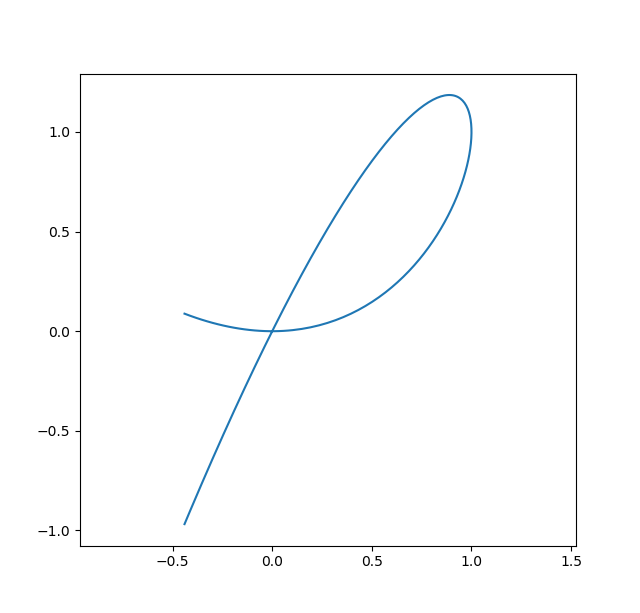
\includegraphics[width = 0.35\textwidth]{1.png}
    \end{center}
  \end{wrapfigure}
\noindent 1. 求由$y^2-2xy+x^3=0$ 所确定的封闭曲线所包围的图形面积.
\begin{proof}[解]
  \noindent 为分析图形形状, 找出$y$随$x$变化的规律, 我们令$y=tx$求得参数曲线
  \[x=2t-t^2,y=2t^2-t^3\]
  $t$从$0$到$2$形成了一段闭曲线. 这段闭曲线所围成的图形面积为
  \begin{eqnarray*}
    S&=&\frac{1}{2}\int_0^2(x\ud y-y\ud x)\\
    &=&\frac{1}{2}\int_0^2[x\ud (2t^2-t^3)-y\ud (2t-t^2)]\\
    &=&\frac{1}{2}\int_0^2(4t^2-4t^3+t^4)\ud t=\frac{8}{15}
  \end{eqnarray*}
\end{proof}

\noindent 2. 设曲线方程为$y=\int_0^x\sqrt{\sin t}\mathrm{d}t, 0\leq x\leq\pi$, 求曲线的长度.
\begin{proof}[解]
  记方程为$y=f(x)$,依据弧长计算公式
  \begin{eqnarray*}
    l&=&\int_0^\pi\sqrt{1+f'(x)^2}\ud x=\int_0^\pi\sqrt{1+\sin x}\\
    &=&\int_0^\pi(\sin\frac{x}{2}+\cos\frac{x}{2})\ud x\\
    &=&4
  \end{eqnarray*}
\end{proof}

\subsection*{作业选讲}

\noindent 22. 设函数 $f(x)\in C(-\infty,+\infty)$, 且 $f'(0)$ 存在, 再设对于
$\forall x\in(-\infty,+\infty),\int_0^xf(t)\mathrm{d}t=\frac{1}{2}xf(x)$.
证明: $f(x)\equiv cx$,其中$c\in\mathrm{R}$为常数.
\begin{proof}
  令$F=\int_0^xf(t)\ud t$, 则$F$在$\mr$上可微, 且$F'=f$,
  从而$f=\frac{2F}{x}$在$\mr/\{0\}$上可微, 由于$f'(0)$存在, 故$f$在
  $\mr$上可微. $f=F'=\frac{1}{2}xf'+\frac{1}{2}f, \forall x\in\mr$
  故$f(x)=xf'(x),\forall x\in\mr$. 对任意不包含$0$的区间$[a,b]$, 有
  \[\ln |f(b)|-\ln |f(a)|=\int_a^b\ud \ln |f(x)|=\int_a^b\frac{f'(x)}{f(x)}\ud x=\int_a^b\frac{1}{x}\ud x=\ln |b|-\ln |a|\]
  故对于$x>0$有$|f(x)|=|f(1)x|$, 对$x<0$有$|f(x)|=|f(-1)x|$. 由$f$在$\mr$上的连续性可知$f(x)=f(1)x,\forall x>0,f(x)=-f(-1)x,\forall x<0$. 再由$f$在$0$处的可微性知$f(x)=f(1)x,\forall x\in\mr$.证毕.
\end{proof}

\noindent 23. 设$P_n(x)$为$n\geq1$次多项式, $[a,b]$是任一闭区间. 证明:
\(\int_a^b|P_n'(x)|\mathrm{d}x\leq2n\max_{a\leq x\leq b}\{|P_n(x)|\}\)
\begin{proof}[提示]
  \ 
  \begin{enumerate}
    \item $|P_n|$的最大值一定是$P_n$的最大值或最小值, 一定是$P_n'$的零点.
    \item $P_n'$的零点至多有$n-1$个.这些零点把$[a,b]$划分成至多
      $n$个区间.
    \item 对于上述任意一个小区间$[s,t]$, $P_n'$在$[s,t]$保持正负不变, 因此$\int_s^t|P_n'(x)|\ud x=|\int_s^tP_n'(x)\ud x|=|P_n(t)-P_n(s)|\leq 2\max_{a\leq x\leq b}|P_n(x)|$
  \end{enumerate}
\end{proof}

\noindent 25. 求下列极限:
\[
(2)\lim_{x\to0+0}\frac{\int_0^x(\sin t)^\alpha\mathrm{d}t}{x^{1+\alpha}};
(3)\lim_{x\to\infty}\frac{\int_0^xe^{t^\alpha}\mathrm{d}t}{x^{1-\alpha}e^{x^\alpha}}(\alpha>0).
\]
\begin{proof}[提示]
  \ 
  \begin{enumerate}
    \setcounter{enumi}{1}
  \item $(\sin t)^\alpha=t^\alpha+o(t^\alpha), \int_0^x(\sin t)^\alpha\ud t=\int_0^xt^\alpha+\int_0^xo(t^\alpha)$
    \item 洛必达法则
  \end{enumerate}
\end{proof}

\noindent 37. (Riemann定理)设函数$f(x)$在区间$[a,b]$上可积, $g(x)$是$(-\infty,+\infty)$上以$T>0$为周期
的连续函数, 且$\int_0^Tg(x)\mathrm{d}x=0$. 证明:
\[
\lim_{\lambda\to\infty}\int_a^bf(x)g(\lambda x)\mathrm{d}x=0
\]
\begin{proof}[作业提示]
  作业中所给的条件是``$f$在区间$[a,b]$单调'', 
  因此作业题可以用定积分第二中值定理来做.
  由于$f$单调, 故
  \begin{eqnarray*}
    \int_a^bf(x)g(\lambda x)\ud x&=&f(a)\int_a^\xi g(\lambda x)\ud x+f(b)\int_\xi^b g(\lambda x)\ud x\\
    &=&f(a)\int_{\xi'}^\xi g(\lambda x)\ud x+f(b)\int_{\xi}^{\xi'+\frac{T}{\lambda}}g(\lambda x)\ud x\\
    &=&\to0 (\text{ as } \frac{T}{\lambda}\to0).
  \end{eqnarray*}
\end{proof}
\begin{proof}
  这里我们将条件放宽为``$f$在$[a,b]$可积'',证明完整的Riemann定理.

  由于$f$可积, 故对任意的$\varepsilon,\sigma>0$, 存在$\delta\in(0,b-a)$, 当
  $\Delta=\frac{T}{\lambda}<\delta$时, $f$在划分
  \[[a,a+\Delta,a+2\Delta,\cdots,a+n\Delta,b],n=[\frac{b}{\Delta}]\]
  下满足$\sum_{i=1}^{n+1}\omega_i\Delta_i<\sigma$, 
  其中$\omega_i(i=1,\cdots,n+1)$是$f$在这$n+1$个区间上的振幅, 
  $\Delta_i=\Delta(i=1,\cdots,n),\Delta_{n+1}=b-a-n\Delta<\Delta$
  是各小区间长.
  
  记$f(x)(x\in[a,b]),g(x)(x\in[0,T])$的绝对值最大值分别是$F,G$.
  记$f$在第$i$个小区间上的最小值为$f_i$.
  对$i=1,\cdots,n$, 由$\int_{a+i\Delta}^{a+(i+1)\Delta}g(\lambda x)\ud x=0$, 
  \begin{eqnarray*}
    \left\vert\int_{a+i\Delta}^{a+(i+1)\Delta}f(x)g(\lambda x)\ud x\right\vert&=&\left|\int_{a+i\Delta}^{a+(i+1)\Delta}(f(x)-f_i)g(\lambda x)\ud x\right|\\
    &\leq&\int_{a+i\Delta}^{a+(i+1)\Delta}|\omega_ig(\lambda x)\ud x|\\
    &\leq&G\cdot\omega_i\Delta_i
  \end{eqnarray*}
  同时$|\int_{a+n\Delta}^{b}f(x)g(\lambda x)\ud x|\leq FG(b-a-n\Delta)\leq FG\Delta$
  故$|\int_a^bf(x)g(\lambda x)\ud x|\leq G\sum_{i=1}^{n+1}\omega_i\Delta_i+FG\Delta\leq G\cdot\sigma+FG\Delta$
\end{proof}

\subsection*{扩展参考}

\subsubsection*{积分的连续性相关问题}

\noindent 1. 设$f\in\mathrm{R}[a,b]$, 证明: 对于每一个给定的$\varepsilon>0$, 存在函数$g$,使得
\[\int_a^b|f(x)-g(x)|\mathrm{d}x<\varepsilon\]
其中$g$是:(1)阶梯函数;(2)折线函数;(3)连续函数;(4)连续可微函数;
\begin{proof}[提示]
  \ 
  \begin{enumerate}
    \item 依据达布理论构造阶梯函数$g_1$
    \item 将阶梯函数在每个小区间边界的更小区间内用折线接起来$g_2$
    \item 折线函数就是连续函数$g_3$
    \item 由于连续函数$g_3$在闭区间一致连续, 
      考虑$g_4(x)=\frac{1}{2\delta}\int_{x-\delta}^{x+\delta}g_3(x)$,
      $g_4$为连续可微函数.
  \end{enumerate}
\end{proof}

\noindent 2. 设$f\in\mathrm{R}[a-\delta,b+\delta]$, 其中$\delta>0$, 则有
  \[\lim_{h\to0}\int_a^b|f(x+h)-f(x)|\mathrm{d}x=0\]
  \begin{proof}[提示]
    使用上面1的结论, 用连续函数$g$逼近$f$, 
    再由$g$的一致连续性得到结论.
  \end{proof}


\subsubsection*{一些简单的渐近分析}

\noindent 1. (例7.5.1)设函数$f(x)\in\mathrm{C}[0,1]$, 则,
    \[
\lim_{n\to\infty}\int_0^1\frac{nf(x)}{1+n^2x^2}\mathrm{d}x=\frac{\pi}{2}f(0)
    \]
  \begin{proof}[讨论]
    上述积分$\int_0^1\frac{nf(x)}{1+n^2x^2}\mathrm{d}x$直观的说
    就是$f(x)$的加权求和/积分, 
    权重是$\frac{n}{1+n^2x^2},(x\in[0,1])$. 当$n$增大时, 
    对于比较大的$x$, 权重可以忽略不计. 所以$n\to\infty$时, 
    积分的极限只与$f(0)$有关. 剩下的就是我们要把这个事情说清楚.

    取$\xi_n$满足当$n\to\infty$时有$\frac{n}{1+n^2\xi_n^2}\to0,\xi_n\to0$,
    例如书中所取的$\xi_n=n^{-\frac{1}{3}}$就符合这个要求.
    再证明
    \[
      \int_0^{\xi_n}\frac{nf(x)}{1+n^2x^2}\mathrm{d}x\approx f(0)\int_0^{\xi_n}\frac{n}{1+n^2x^2}\ud x\to\frac{\pi}{2}f(0),
      \int_{\xi_n}^1\frac{nf(x)}{1+n^2x^2}\mathrm{d}x\to0
    \]
    
  \end{proof}

\noindent 2. 求证$\lim_{n\to\infty}\int_0^1(1-x^2)^n\mathrm{d}x=0$.
  \begin{proof}[提示]
    取$\xi_n$满足$\xi_n\to0,(1-\xi_n^2)^n\to0$, 例如$\xi_n=n^{-\frac{1}{3}}$就符合这个要求. 再分别证明:
    \[\int_0^{\xi_n}(1-x^2)^n\ud x\to0,\int_{\xi_n}^1(1-x^2)^n\ud x\to0\]
  \end{proof}

\noindent 3. 对$[a,b]$上的实值函数$f,\phi$, 定义, 
    \(
    I(x)=\int_a^bf(t)e^{x\phi(t)}\mathrm{d}t
    \)
  为了简化讨论, 我们这里假设$f,\phi$具有无穷阶导数, 且$\phi'$在$(a,b)$上大于0. $f(b)>0$.
请描述上述积分$I$随着$x\to\infty$的渐近行为. 

  在这里我们并没有严格定义``渐近行为''是什么意思, 简单来说, 
  这个问题是希望我们给出一个简单的关于$I(x)$的近似公式. 
  至于有多近似, 近似到多少阶, 则是开放性的事情了. 
  下面我们着重讲两种方法.
  \begin{proof}[method 1: 局部分析-Laplace方法]
    为了后面叙述方便, 记$\phi^1=\phi'(b),\phi^2=\phi''(b),F_0=f(b)e^{x\phi(b)}$.
    我们先待定一个无穷小量$\varepsilon_x$, 这个$\varepsilon_x$随着$x\to\infty$而
    趋向于$0$, 而$\varepsilon_x$以何种速度趋向于$0$则取决与具体情形. 在这里,
    我们就取$\varepsilon_x=x^{-\frac{2}{3}}$, 
    至于为何这么取, 我们看后面的分析过程就自然知道.
    
    依据$\varepsilon_x$的取法, 我们知道, 当$t\leq b-\varepsilon_x$, 
    $x(\phi(b-\frac{\varepsilon_x}{2})-\phi(t))\geq
    x(\phi(b-\frac{\varepsilon_x}{2})-\phi(b-\varepsilon_x))
    \sim\frac{\phi^1}{2}x^{\frac{1}{3}}$
    从而$
    \int_{0}^{b-\varepsilon_x}f(t)e^{x\phi(t)}\mathrm{d}t
    =o(\int_{b-\frac{\varepsilon_x}{2}}^{b}f(t)e^{x\phi(t)}\mathrm{d}t)$, 因此
    \[
      I(x)\sim\int_{b-\varepsilon_x}^bf(t)e^{x\phi(t)}\mathrm{d}t,
      x\to\infty,
    \]

    又由于$f(t)$ 连续, 我们有
    $\int_{b-\varepsilon_x}^bf(t)e^{x\phi(t)}\mathrm{d}t \sim \int_{b-\varepsilon_x}^bf(b)e^{x\phi(t)}\mathrm{d}t$
    从而
    \[
      I(x)\sim\int_{b-\varepsilon_x}^bf(b)e^{x\phi(t)}\mathrm{d}t,
      x\to\infty,
      \]
    在$b$附近$\phi(t)=\phi(b)+\phi^1\cdot(t-b)+\frac{\phi^2}{2}\cdot(t-b)^2+O((t-b)^3)$,
    为了方便讨论, 我们在$b$附近做变量替换, 于是有
    \[
      I(x)\sim 
      F_0\int_0^{\varepsilon_x}e^{-\phi^1xt+\frac{\phi^2x}{2}t^2+xO(t^3)}\ud t,x\to\infty
      \]
    由$\varepsilon_x=x^{-\frac{2}{3}}$, $\frac{\phi^2x}{2}t^2+xO(t^3)=o(1)$, 
    从而$e^{-\phi^1xt+\frac{\phi^2x}{2}t^2+xO(t^3)}=e^{-\phi^1xt}+o(e^{-\phi^1xt}),
    \forall 0\leq t\leq\varepsilon_x$, 故
    \[
      I(x)\sim F_0\int_0^{\varepsilon_x}e^{-\phi^1xt}\ud t,
      x\to\infty,
      \]
    做变量替换$s=xt$, 于是
    $\int_0^{x^{-\frac{2}{3}}}e^{-\phi^1xt}\ud t=
    \frac{1}{x}\int_0^{x^\frac{1}{3}}e^{-\phi^1s}\ud s
    =-\frac{1}{\phi^1x}
    \left.e^{-\phi^1s}\right|_0^{x^\frac{1}{3}}$,
    由$e^{-\phi^1x^{\frac{1}{3}}}=o(\frac{1}{x})$, 
    因此最终得到
    \[I(x)\sim \frac{f(b)}{\phi'(b)x}e^{x\phi(b)}\]
    
    回顾上面的分析过程, 我们可以知道, 只要$\varepsilon_x$满足
    \[\varepsilon_x\to0,x\varepsilon_x\to\infty,x\varepsilon_x^2\to0\]
    那么上面的分析都仍然正确.
  \end{proof}
  \begin{proof}[method 2: 基于分部积分]
    \begin{eqnarray*}
      I(x)&=&\frac{1}{x}\int_a^b\frac{f(t)}{\phi'(t)}\frac{\ud}{\ud t}e^{x\phi(t)}\\
      &=&\left.\frac{1}{x}\frac{f(t)}{\phi'(t)}e^{x\phi(t)}\right\vert_a^b
      -\frac{1}{x}\int_a^b\frac{\ud}{\ud t}\left[\frac{f}{\phi'}\right]e^{x\phi(t)}\ud t\\
      &\sim&\frac{1}{x}\frac{f(b)}{\phi'(b)}e^{x\phi(b)}
    \end{eqnarray*}
    由此我们得到了$I(x)$随着$x\to\infty$的渐近行为.

    更进一步, 用同样的方法我们可以依次求出$A_1,A_2,\cdots$, 
    使得对任意的$n\in\mn$, 有
    \[I(x)\sim e^{x\phi(b)}\sum_{i=1}^{n}A_ix^{-i}\]

    需要注意到, 上面得到
    $I(x)\sim \frac{f(b)}{\phi'(b)x}e^{x\phi(b)}$
    的这一步本身仍然不够经得起推敲, 仍然需经过前面的Laplace方法
    才能得到结论. 并不能说这里可以得到$I(x)$的各阶逼近就说明这个方法更好, 
    基于分部积分的方法与Laplace局部分析方法的所用到的思想和技巧对于
    分析来说都是基础而重要的.
  \end{proof}


%\begin{algorithm}
%  \caption*{ADMM求解$\min_{X\succeq0}|X|_1,\st |SX-I|\leq\sigma$}
%  %  \caption{ADMM求解$\min_{X\succeq0}|X|_1,\st |SX-I|\leq\sigma$}\label{alg:ADMM}
%  \begin{algorithmic}
%    \Require $S,\sigma,\rho$
%    \Ensure $X,|X|_1$
%    \State \textbf{Repeat while not convergence}
%    \begin{enumerate}
%      \item  根据式(\ref{eq:updateW3_2}
%      $\sim$\ref{eq:updateZ3_2}),依次求$W^+,X^+,Y^+,Z^+$;
%      \item  根据式(\ref{eq:updateU3_2}),依次求${U^1}^+,{U^2}^+,{U^3}^+$;
%    \end{enumerate}
%    \Return $X,|X|_1$
%  \end{algorithmic}
%\end{algorithm}

%\begin{lstlisting}[language=Matlab,keywordstyle=\color{blue},commentstyle=\color{red!80!green!80!blue!80}, rulesepcolor=\color{red!50!green!50!blue!50},tabsize=4]
%
%\end{lstlisting}

%\begin{figure}[htbp!]
%\centering
%\makebox[\textwidth][c] {
%\includegraphics[width=0.9\paperwidth]{}
%}
%\caption{}\label{}
%\end{figure}
%
%\begin{figure}[htbp!]
%   \centering
%   \begin{subfigure}{.48\textwidth}
%	\centering
%	\includegraphics[width = \textwidth]{}
%	\caption{} \label{}
%   \end{subfigure} 
%   \begin{subfigure}{.48\textwidth}
%	\centering
%	\includegraphics[width = \textwidth]{}
%	\caption{} \label{}
%   \end{subfigure}
%   \caption{} \label{}
%\end{figure}

%\begin{table}[htbp!]
%\centering
%\caption{} 
%\begin{subfigure}{0.49\textwidth}
%   \centering
%   \caption{}
%   \begin{tabular}{}
%
%   \end{tabular}
%\end{subfigure}
%\begin{subfigure}{.49\textwidth}
%   \centering
%   \caption{} 
%   \begin{tabular}{}
%
%   \end{tabular}    
%\end{subfigure}
%\end{table}

%\begin{centering}
%\section*{致谢}\addcontentsline{toc}{section}{致谢}
%\end{centering}

%\newpage
%\begin{thebibliography}{}
%\addcontentsline{toc}{section}{参考文献}
%\bibitem{cite_ADMM}Boyd S, Parikh N, Chu E, et al. Distributed Optimization and Statistical Learning via the Alternating Direction Method of Multipliers[J]. Foundations \& Trends® in Machine Learning, 2011, 3(1):1-122.
%\bibitem{cite_FISTA}Beck A, Teboulle M. A Fast Iterative Shrinkage-Thresholding Algorithm for Linear Inverse Problems[J]. Siam Journal on Imaging Sciences, 2009, 2(1):183-202.
%\bibitem{cite_convexoptimization}Boyd S, Vandenberghe L. Convex Optimization[M]. Cambridge University Press, 2004.
%%\bibitem{cite_quasicrystalsgreen}刘有延,傅秀军.\emph{准晶体}[M]. 上海科技教育出版社,1999.
%\end{thebibliography}

\bibliography{ref}
\end{document}



